\documentclass{article}% or something else
\usepackage{pdfpages}

\usepackage{soul}


\begin{document}


\section{Review for DATA 301 Midterm 2}

This is what the midterm looks like last year.  I am not bound to the exact percentages, but they should give you a rough idea on how to study.

\subsection{Proposed Format}

Time limit: 80 minutes\\
Total marks: 30\\

\begin{itemize}
\item $\sim$ 15 multiple choice (MC) questions   (30 minutes total -- 15 marks)
\item $\sim$  3 of 4 small programming questions (30 minutes total--- 15 marks)
%- Up to 2 bonus marks for any of the programming questions
\end{itemize}


\subsection{Topic Breakdown}

\begin{itemize}
\item  100\% - Python
\end{itemize}


%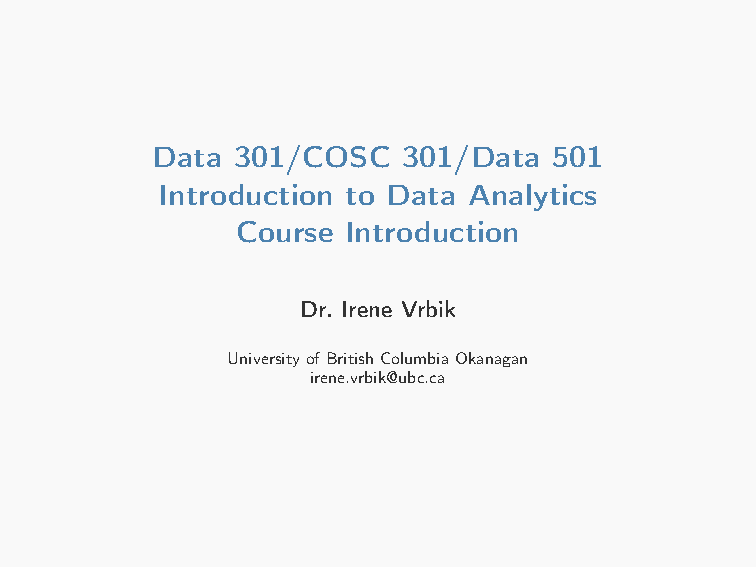
\includepdf[pages=-]{01Intro}
%\includepdf[pages=-]{02DataRepresentation.pdf}
%\includepdf[pages=-]{03ExcelPartIBeamer.pdf}
%\includepdf[pages=-]{03ExcelPartII.pdf}
%
\includepdf[pages=-]{04ExcelVBA.pdf}
%\includepdf[pages=-]{05Databases.pdf}
%\includepdf[pages=-]{05DatabasesII.pdf}
%\includepdf[pages=-]{06CommandLine.pdf}


\section{List of Topics}


\begin{table}[h]
\caption{Key}
\begin{center}
\begin{tabular}{|c|l|}
\hline
{\tt ***} & Extremely important\\
 {\tt **} & Assignment question or major topic\\
  {\tt *} &Important topic which probably should be tested\\
    -& (no stars) topic covered but of minor importance\\
   \st{strikethrough} & Important but not testable for this midterm\\ 
\hline
\end{tabular}
\end{center}
\label{default}
\end{table}%



\subsection*{07Python (part I and II)}

\begin{itemize}
\item[-] Jupyter Notebook
\item[*] Explain what is Python and note the difference between Python 2 and 3
\item[*]  Python data types (see using {\tt type} function)
\item[*] Define: algorithm, program, language, programming
\item[**] Follow Python basic syntax rules including indentation/comments
\item[***] Define and use variables and assignment
\item[*] Apply Python variable naming rules
\item[*] Perform math expressions and understand operator precedence
\item[***] Use strings, character indexing, string functions
\item[**] String functions: split, substr, concatenation
\item[**] Importing  Python modules
\item[*] Use Python datetime and clock functions
\item[***] Read input from standard input (keyboard)
\item[***] Create comparisons and use them for decisions with if
\item[***] Combine conditions with and, or, not
\item[***] Use if/elif/else syntax
\item[***] Looping with for and while (eg. with {\tt range} or with Python lists, strings., etc.)
\item[***] Create and use lists and list functions/methods
\item[**] Differences between functions and methods
\item[-]  Advanced: list comprehensions, list slicing
\item[***] Create and use dictionaries
\item[*] Create and use tuples and sets 
\item[*] Differences between lists, tuples, sets and dictionaries
\item[***] Print formatting 
\item[***] Create and use Python functions
\item[-] Difference between Python functions and procedures
\item[*] Use built-in functions in math library
\item[*] Create random numbers
\item[-] Advanced: passing functions, lambda functions
\end{itemize}


\subsection*{07Python (part I)}


\begin{itemize}
\item[***] Open, read, write, append
\item[**] Closing files (either in a {\tt with} clause or using {\tt fileobj.close()})
\item[***] Process CSV files
\item[*]   Using the csv module (you can use this module if you like but you don't have too)
\item[**] Define: exception, exception handling
\item[***] Use try-except statement to handle exceptions and understand how each of try, except, else, finally blocks are used
\item[-] Define: IPv4/IPv6 address, domain, domain name, URL
\item[*] Read URLs using urllib.request.
%\item[**] \st{Use Biopython module to retrieve NCBI data and perform BLAST}
%\item[**] Build charts using matplotlib
%\item[*] Perform linear regression and k-means clustering using SciPy
%\item[*] Connect to and query the MySQL database using Python
%\item[*] Write simple Map-Reduce programs
\end{itemize}



%\subsection*{Title}
%
%\begin{itemize}
%    \item[-] 
%\item[*]
%\item[**]
%\item[***]
%\end{itemize}








\end{document}